%\documentclass[hyperref={pdfpagelabels=false},slidetop,9pt]{beamer}
\documentclass[slidetop,8pt]{beamer}
\usepackage[T1]{fontenc}
\usepackage[utf8]{inputenc}
\newcommand{\id}{54}
\newcommand{\nom}{Liaisons mécaniques}
\newcommand{\sequence}{04}
\newcommand{\num}{01}
\newcommand{\type}{TP}
\newcommand{\descrip}{Modélisation d'un solide. Comportement des liaisons mécaniques. Modéliser les mécanismes du laboratoire par un schéma cinématique, paramétré.}
\newcommand{\competences}{A3-C4: Analyse d'architecture et de comportement \\ &  Mod1-C1: Isolement d'un solide ou d'un système de solides \\ &  Mod2-C10-1: Modèle de solide indéformable \\ &  Mod2-C11: Modélisation géométrique et cinématique des mouvements entre solides indéformables \\ &  Mod2-C12: Modélisation cinématique des liaisons entre solides \\ &  Mod2-C15: Modélisation des actions mécaniques \\ &  Rés-C6: Utilisation d'un solveur ou d'un logiciel multi physique \\ &  Com1-C1: Différents descripteurs introduits dans le programme \\ &  Com2-C4: Outils de communication}
\newcommand{\nbcomp}{9}
\newcommand{\systemes}{Plateforme Stewart}
\newcommand{\systemessansaccent}{Plateforme Stewart}
\newcommand{\ilot}{2}
\newcommand{\ilotstr}{02}
\newcommand{\dossierilot}{\detokenize{Ilot_02 Plateforme Stewart}}
\newcommand{\imageun}{Plateforme}

\newcommand{\urlsysteme}{\href{https://www.costadoat.fr/systeme/57}{Ressources système}}
\newcommand{\matlabsimscape}{\href{https://github.com/Costadoat/Sciences-Ingenieur/raw/master/Systemes/Plateforme Stewart/Plateforme_Stewart_Simscape.zip}{Modèle Simscape}}
\newcommand{\solidworks}{\href{https://github.com/Costadoat/Sciences-Ingenieur/raw/master/Systemes/Plateforme Stewart/Plateforme_Stewart_Solidworks.zip}{Modèle Solidworks}}
\newcommand{\edrawings}{\href{https://github.com/Costadoat/Sciences-Ingenieur/raw/master/Systemes/Plateforme Stewart/Plateforme_Stewart.EASM}{Modèle eDrawings}}
\newcommand{\test}{Stewart_param1}
\newcommand{\testi}{Stewart_param2}
\newcommand{\testii}{Stewart_param3}
\newcommand{\testiii}{Stewart_param4}
\newcommand{\testiiii}{Stewart_euler}
\usepackage{etex}
\usepackage{tikz}
\usepackage[european]{circuitikz}
\usepackage{pgf}
\usepackage[all]{xy}
\usepackage{pgfpages}
\usepackage{graphbox}
\usepackage{pdfpages}
\usepackage[adobe-utopia]{mathdesign}
\usepackage{ifthen}
\usepackage{cancel}
\usepackage{framed}
\usepackage{subfig}
\usepackage{tabularx}
\usepackage{setspace}
\usepackage{soul}
\usepackage{schemabloc}
\usepackage{eqnarray}
\usepackage[dot, phantomtext]{dashundergaps}
\usepackage{media9}
\usepackage{multimedia}
\usepackage{textcomp}

\author{Renaud Costadoat}
\institute{Lycée Dorian}

\usepackage{multido}
\usepackage{multirow}
\usepackage{multicol} % Portions de texte en colonnes
\usepackage{flafter}%floatants après la référence

\usepackage{color}
\usepackage{xcolor}
\usepackage{colortbl}

\usepackage[gen]{eurosym}
\usepackage{tikz}
%\usepackage{pstricks,pst-node,pst-tree,pst-solides3d}
\usepackage{lmodern}
\usepackage[francais]{babel}
\usepackage{pslatex}
\usetheme{renaud}
\usepackage{times}
\usepackage{amsmath}
\usepackage{verbatim}
\usepackage{moreverb}
%\usetikzlibrary{arrows,shapes}
\usepackage{graphicx}
\usepackage{psfrag}
\usepackage{wrapfig}
\usepackage{etoolbox}

\definecolor{gris25}{gray}{0.75}
\definecolor{bleu}{RGB}{18,33,98}
\definecolor{bleuf}{RGB}{42,94,171}
\definecolor{bleuc}{RGB}{231,239,247}
\definecolor{rougef}{RGB}{185,18,27}
\definecolor{rougec}{RGB}{255,188,204}%255,230,231
\definecolor{vertf}{RGB}{103,126,82}
\definecolor{vertc}{RGB}{220,255,191}

\setlength\parindent{24pt}
\parskip 7.2pt
\parindent 8pt

\newenvironment{rem}[1][\hsize]%
{%
    \def\FrameCommand
   {%
\rotatebox{90}{\textit{\textsf{Remarque}}} 
       {\color{bleuf}\vrule width 3pt}%
       \hspace{0pt}%must no space.
       \fboxsep=\FrameSep\colorbox{bleuc}%
  }%
    \MakeFramed{\hsize#1\advance\hsize-\width\FrameRestore}%
}%
{\endMakeFramed}%


\newenvironment{savoir}[1][\hsize]%
{%
    \def\FrameCommand
    {%
\rotatebox{90}{\textit{\textsf{Savoir}}} 
        {\color{bleuf}\vrule width 3pt}%
        \hspace{0pt}%must no space.
        \fboxsep=\FrameSep\colorbox{bleuc}%
    }%
    \MakeFramed{\hsize#1\advance\hsize-\width\FrameRestore}%
}%
{\endMakeFramed}%

\newenvironment{prob}[1][\hsize]%
{%
    \def\FrameCommand%
    {%
\rotatebox{90}{\textit{\textsf{Problematique}}} 
        {\color{rougef}\vrule width 3pt}%
        \hspace{0pt}%must no space.
        \fboxsep=\FrameSep\colorbox{rougec}%
    }%
    \MakeFramed{\hsize#1\advance\hsize-\width\FrameRestore}%
}%
{\endMakeFramed}%

\newenvironment{obj}[1][\hsize]%
{%
    \def\FrameCommand%
    {%
\rotatebox{90}{\textit{\textsf{Objectif}}} 
        {\color{vertf}\vrule width 3pt}%
        \hspace{0pt}%must no space.
        \fboxsep=\FrameSep\colorbox{vertc}%
    }%
    \MakeFramed{\hsize#1\advance\hsize-\width\FrameRestore}%
}%
{\endMakeFramed}%

\newenvironment{defi}[1][\hsize]%
{%
    \def\FrameCommand%
    {%
\rotatebox{90}{\textit{\textsf{Definition}}} 
        {\color{bleuf}\vrule width 3pt}%
        \hspace{0pt}%must no space.
        \fboxsep=\FrameSep\colorbox{rougec}%
    }%
    \MakeFramed{\hsize#1\advance\hsize-\width\FrameRestore}%
}%
{\endMakeFramed}%


\newenvironment{hypo}[1][\hsize]%
{%
    \def\FrameCommand%
    {%
\rotatebox{90}{\textit{\textsf{Hypothèse\\}}} 
        {\color{bleuf}\vrule width 3pt}%
        \hspace{0pt}%must no space.
        \fboxsep=\FrameSep\colorbox{bleuc}%
    }%
    \MakeFramed{\hsize#1\advance\hsize-\width\FrameRestore}%
}%
{\endMakeFramed}%


\newenvironment{prop}[1][\hsize]%
{%
    \def\FrameCommand%
    {%
\rotatebox{90}{\textit{\textsf{Propriété}}} 
        {\color{bleuf}\vrule width 3pt}%
        \hspace{0pt}%must no space.
        \fboxsep=\FrameSep\colorbox{bleuc}%
    }%
    \MakeFramed{\hsize#1\advance\hsize-\width\FrameRestore}%
}%
{\endMakeFramed}%

\newenvironment{props}[1][\hsize]%
{%
    \def\FrameCommand%
    {%
\rotatebox{90}{\textit{\textsf{Propriétés}}} 
        {\color{bleuf}\vrule width 3pt}%
        \hspace{0pt}%must no space.
        \fboxsep=\FrameSep\colorbox{bleuc}%
    }%
    \MakeFramed{\hsize#1\advance\hsize-\width\FrameRestore}%
}%
{\endMakeFramed}%

\newenvironment{exemple}[1][\hsize]%
{%
    \def\FrameCommand%
    {%
\rotatebox{90}{\textit{\textsf{Exemple}}} 
        {\color{vertf}\vrule width 3pt}%
        \hspace{0pt}%must no space.
        \fboxsep=\FrameSep\colorbox{vertc}%
    }%
    \MakeFramed{\hsize#1\advance\hsize-\width\FrameRestore}%
}%
{\endMakeFramed}%

\newenvironment{resultat}[1][\hsize]%
{%
    \def\FrameCommand%
    {%
\rotatebox{90}{\textit{\textsf{Résultat}}} 
        {\color{rougef}\vrule width 3pt}%
%        {\color{bleuf}\vrule width 3pt}%
        \hspace{0pt}%must no space.
        \fboxsep=\FrameSep\colorbox{rougec}%
    }%
    \MakeFramed{\hsize#1\advance\hsize-\width\FrameRestore}%
}%
{\endMakeFramed}%

\newenvironment{methode}[1][\hsize]%
{%
    \def\FrameCommand%
    {%
\rotatebox{90}{\textit{\textsf{Méthode\\}}} 
        {\color{rougef}\vrule width 3pt}%
        \hspace{0pt}%must no space.
        \fboxsep=\FrameSep\colorbox{rougec}%
    }%
    \MakeFramed{\hsize#1\advance\hsize-\width\FrameRestore}%
}%
{\endMakeFramed}%

\newenvironment{theo}[1][\hsize]%
{%
    \def\FrameCommand%
    {%
\rotatebox{90}{\textit{\textsf{Théorème\\}}} 
        {\color{rougef}\vrule width 3pt}%
        \hspace{0pt}%must no space.
        \fboxsep=\FrameSep\colorbox{rougec}%
    }%
    \MakeFramed{\hsize#1\advance\hsize-\width\FrameRestore}%
}%
{\endMakeFramed}%

\newenvironment{warn}[1][\hsize]%
{%
    \def\FrameCommand%
    {%
\rotatebox{90}{\textit{\textsf{Attention\\}}} 
        {\color{rougef}\vrule width 3pt}%
        \hspace{0pt}%must no space.
        \fboxsep=\FrameSep\colorbox{rougec}%
    }%
    \MakeFramed{\hsize#1\advance\hsize-\width\FrameRestore}%
}%
{\endMakeFramed}%

% \usepackage{pstricks}
%\usepackage{minitoc}
% \setcounter{minitocdepth}{4}

\setcounter{tocdepth}{2}

% \mtcselectlanguage{french} 

%\usepackage{draftcopy}% "Brouillon"
% \usepackage{floatflt}
\usepackage{psfrag}
%\usepackage{listings} % Permet d'insérer du code de programmation
\renewcommand{\baselinestretch}{1.2}

% Changer la num�rotation des figures :
% ------------------------------------
% \makeatletter
% \renewcommand{\thefigure}{\ifnum \c@section>\z@ \thesection.\fi
%  \@arabic\c@figure}
% \@addtoreset{figure}{section}
% \makeatother
 


%%%%%%%%%%%%
% Définition des vecteurs %
%%%%%%%%%%%%
 \newcommand{\vect}[1]{\overrightarrow{#1}}

%%%%%%%%%%%%
% Définition des torseusr %
%%%%%%%%%%%%

 \newcommand{\torseur}[1]{%
\left\{{#1}\right\}
}

\newcommand{\torseurcin}[3]{%
\left\{\mathcal{#1} \left(#2/#3 \right) \right\}
}

\newcommand{\torseurstat}[3]{%
\left\{\mathcal{#1} \left(#2\rightarrow #3 \right) \right\}
}

 \newcommand{\torseurc}[8]{%
%\left\{#1 \right\}=
\left\{
{#1}
\right\}
 = 
\left\{%
\begin{array}{cc}%
{#2} & {#5}\\%
{#3} & {#6}\\%
{#4} & {#7}\\%
\end{array}%
\right\}_{#8}%
}

 \newcommand{\torseurcol}[7]{
\left\{%
\begin{array}{cc}%
{#1} & {#4}\\%
{#2} & {#5}\\%
{#3} & {#6}\\%
\end{array}%
\right\}_{#7}%
}

 \newcommand{\torseurl}[3]{%
%\left\{\mathcal{#1}\right\}_{#2}=%
\left\{%
\begin{array}{l}%
{#1} \\%
{#2} %
\end{array}%
\right\}_{#3}%
}

 \newcommand{\vectv}[3]{%
\vect{V\left( {#1} \in {#2}/{#3}\right)}
}


\newcommand{\vectf}[2]{%
\vect{R\left( {#1} \rightarrow {#2}\right)}
}

\newcommand{\vectm}[3]{%
\vect{\mathcal{M}\left( {#1}, {#2} \rightarrow {#3}\right)}
}


 \newcommand{\vectg}[3]{%
\vect{\Gamma \left( {#1} \in {#2}/{#3}\right)}
}

 \newcommand{\vecto}[2]{%
\vect{\Omega\left( {#1}/{#2}\right)}
}

\newcommand{\reponse}[1][4]
{
\multido{}{#1}
{
\begin{center}
\makebox[0.9\linewidth]{\dotfill} \end{center}
}}


% }$$\left\{\mathcal{#1} \right\}_{#2} =%
% \left\{%
% \begin{array}{c}%
%  #3 \\%
%  #4 %
% \end{array}%
% \right\}_{#5}}


%  ------------------------------------------
% | Modification du formatage des sections : | 
%  ------------------------------------------

% Grands titres :
% ---------------

\newcommand{\titre}[1]{%
\begin{center}
      \bigskip
      \rule{\textwidth}{1pt}
      \par\vspace{0.1cm}
      
      \textbf{\large #1}
      \par\rule{\textwidth}{1pt}
    \end{center}
    \bigskip
  }

% Supprime le numéro du chapitre dans la numérotation des sections:
% -----------------------------------------------------------------
\makeatletter
\renewcommand{\thesection}{\@arabic\c@section}
\makeatother


% \titleformat{\chapter}[display]
% {\normalfont\Large\filcenter}
% {}
% {1pc}
% {\titlerule[1pt]
%   \vspace{1pc}%
%   \Huge}[\vspace{1ex}%
% \titlerule]


%%%% Chapitres Comme PY Pechard %%%%%%%%%
% numéro du chapitre
\DeclareFixedFont{\chapnumfont}{OT1}{phv}{b}{n}{80pt}
% pour le mot " Chapitre "
\DeclareFixedFont{\chapchapfont}{OT1}{phv}{m}{it}{40pt}
% pour le titre
\DeclareFixedFont{\chaptitfont}{T1}{phv}{b}{n}{25pt}

\definecolor{gris}{gray}{0.75}
\setbeamertemplate{section in toc}[sections numbered]

\newlength{\RoundedBoxWidth}
\newsavebox{\GrayRoundedBox}
\newenvironment{GrayBox}[1][\dimexpr\textwidth-4.5ex]%
   {\setlength{\RoundedBoxWidth}{\dimexpr#1}
    \begin{lrbox}{\GrayRoundedBox}
       \begin{minipage}{\RoundedBoxWidth}}%
   {   \end{minipage}
    \end{lrbox}
    \begin{center}
    \begin{tikzpicture}%
       \draw node[draw=bleuf,fill=bleuc,rounded corners,%
             inner sep=2ex,text width=\RoundedBoxWidth]%
             {\usebox{\GrayRoundedBox}};
    \end{tikzpicture}
    \end{center}}
    
\ifdef{\prive}{\pgfpagesuselayout{2 on 1}[a4paper,border shrink=0mm]}
\ifdef{\prive}{\setbeamertemplate{navigation symbols}{}}
\setbeamertemplate{itemize item}[ball]
%\setbeamertemplate{blocks}[rounded]%[shadow=true]
\setbeamercolor{block title}{fg=white,bg=grisf}        % titre block normal 
\setbeamercolor{block body}{fg=grisf,bg=grisc!50}      % corps block normal
\setbeamercolor{block body alerted}{fg=white,bg=warning}   % idem pour un block alerte

\title{\nom}
\date{S\sequence \ - \type\num}

\begin{document}
\shorthandoff{:!}
\bibliographystyle{abbrvnat-fr}

\usebackgroundtemplate%
{%
    \centering
\includegraphics[width=\paperwidth]{../../img/fond2}%
}

{
\setbeamertemplate{navigation symbols}{}
\setbeamertemplate{headline}[pagetitre]
\setbeamertemplate{footline}[pagetitre]
\usebackgroundtemplate{\centering
\includegraphics[width=\paperwidth]{../../img/fond}}
\frame{\titlepage}
}



\section{Introduction}

{\frame{
\frametitle{Introduction}

\begin{savoir}
Vous êtes capables :
\begin{itemize}
 \item de déterminer un cahier des charges.
\end{itemize}
\end{savoir}

\begin{prob}
Vous devez êtes capables :
\begin{itemize}
 \item de déterminer les caractéristiques d'un matériaux qui réspondent à un besoin,
 \item de connaître les moyens de déterminer les caractéristiques d'un matériau.
\end{itemize}
\end{prob}
}}

{\frame{
\frametitle{Propriétés et définitions}

\textbf{L'élasticité:} Aptitude d'un corps de subir des déformations temporaires sous charge.

\textbf{La ténacité:} Aptitude d'un corps de résister à la déformation ou à la rupture sous un effort continu.

\textbf{La dureté:} Aptitude d'un corps de résister à la pénétration d'un autre corps et de résister à l'usure.

\textbf{La résilience:} Aptitude à subir des efforts brusques ou des chocs sans rupture.

\textbf{L'endurance:} Aptitude d'un corps de subir des efforts variables et répétés en grandeur et direction.

\textbf{La plasticité:} Aptitude d'un corps à la déformation sans tension ni rupture.

\textbf{La ductilité:} Aptitude d'un corps de pouvoir être étiré sous forme de fils minces.

\textbf{La fluidité:} Aptitude d'un corps d'être porté à fusion et de remplir facilement le moule dans lequel il est coulé (pièces de fonderie).

}}

{\frame{
\frametitle{Propriétés et définitions}

\textbf{Homogénéité:} Un matériau est homogène s'il possède, en tous points, les mêmes propriétés chimiques et physiques. 

\textbf{Isotropie:} Un matériau est isotrope s'il présente les mêmes caractéristiques mécaniques dans toutes les directions de la matière.

\textbf{Contraintes (unités: N/mm2 ou MPa):} Elles caractérisent par des indications chiffrées les efforts de cohésion qui existent entre les grains de matières. Elles peuvent être normales ou de tension, ayant pour symbole $\sigma$ et des contraintes de cisaillement, ayant pour symbole $\tau$.

\textbf{Déformations:} Elles résultent et varient avec les charges  appliquées sur les objets. Elles sont mises en évidence par la variation des dimensions, et peuvent être élastiques ou plastiques.
Ex: allongement, raccourcissement, fléchissement, torsion, glissement,...
}}

{\frame{
\frametitle{Les essais mécaniques}

\begin{itemize}
 \item Les \textbf{essais mécaniques} sont des \textbf{expériences} dont le but est de caractériser les \textbf{lois de comportements} des matériaux (mécanique des milieux continus).
 \item La loi de comportement établit une relation entre les \textbf{contraintes} (pression=force/surface) et les \textbf{déformations} (allongement unitaire sans dimensions). 
\begin{itemize}
 \item \textit{Remarque: Il ne faut pas confondre une déformation avec un déplacement ou une dilatation.}
\end{itemize}
 \item Cependant, la déformation d'une pièce dépend de la forme de la pièce et de la manière dont sont exercés les efforts extérieurs sur cette pièce. Il faut donc normaliser les essais. Des normes définissent donc :
 \begin{itemize}
  \item quelle est la \textbf{forme} de la pièce d'essai dont on teste le matériau, on parle alors \textbf{d'éprouvette normalisée}, 
  \item comment sont exercés les \textbf{efforts} sur l'éprouvette, on parle alors \textbf{d'essai normalisé}.
 \end{itemize}
\end{itemize}
}}

\section{Essai de traction}

{\frame{
\frametitle{Essai de traction}

Une \textbf{éprouvette} est tenue en deux points. Elle est étirée à vitesse constante, et on relève la force de traction nécessaire en fonction de l'allongement. Ces essais permettent de tracer une courbe dite de traction à partir de laquelle les caractéristiques suivantes peuvent être déduites :
\begin{itemize}
 \item la déformation élastique en fonction de la force appliquée d'où on peut déduire, connaissant les dimensions de l'éprouvette, le \textbf{module d'Young},
 \item la \textbf{limite élastique} souvent notée $Re$, ou bien la limite d'élasticité à $0,2\% Re_{0,2}$
 \item la \textbf{déformation plastique}
 \item la \textbf{résistance à la traction} ou tension de rupture souvent notée $R_m$, qui est la contrainte maximale atteinte en cours d'essais.
 \end{itemize}

\begin{minipage}{0.6\linewidth}
L'éprouvette peut être un barreau cylindrique (système symétrique)ou plate (étude d'une face). 

Les extrémités de l'éprouvette sont élargies, avec un congé, afin d'être sûr que la déformation plastique et la rupture auront lieu dans la partie centrale de l'éprouvette.
\end{minipage}
\hfill
\begin{minipage}{0.3\linewidth}
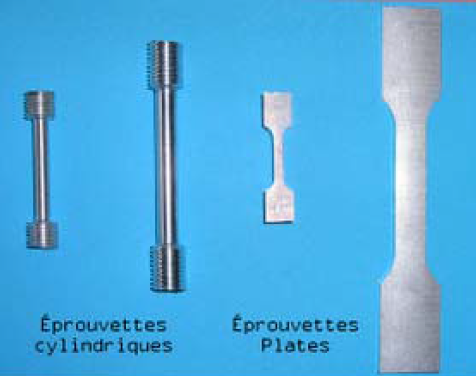
\includegraphics[width=0.9\linewidth]{img/img1}
\end{minipage}
}}

{\frame{
\frametitle{Déroulement de l'essai de traction}

\begin{enumerate}
 \item Suppression du jeu grâce à une légère pré-charge
 \item Etirement de l'éprouvette par un déplacement de la travée
  \begin{itemize}
   \item Mesures :  effort généré par ce déplacement
   \item Remarque: le mouvement peut se faire par un système de vis sans fin ou un piston hydraulique, l'effort se mesure par un capteur d'effort.
  \end{itemize}
 \item Durant le déplacement de la travée
  \begin{itemize}
   \item Calcul: Déformation conventionnelle $\epsilon_c=\frac{\Delta l}{l_0}$ à partir du déplacement et contrainte conventionnelle $\sigma_c=R=\frac{F}{S_0}$ en divisant la force par la section initiale $S_0$ à partir de la force.
  \end{itemize}
 \item L'essai s'arrête à la rupture de l'éprouvette.
\end{enumerate}

Le diagramme ainsi obtenu est appellé \og Diagramme conventionnel \fg.

A partir de ces relevés et en prenant en compte la variation de la section $S$, il est posible de tracer le \og Diagramme rationnel \fg affichant $\sigma_r=\frac{F}{S}=\sigma_c.(1+\epsilon_c)$ en fonction de $\epsilon_r=\int_{L_0}^L\frac{dl}{l}=ln(1+\epsilon_c)$.
}}

{\frame{
\frametitle{Caractéristiques de l'essai de traction}

\begin{defi}
\begin{minipage}{0.7\linewidth}
\begin{itemize}
 \item \textbf{Re: limite d'élasticité} ($MPa$),
 \item Fe: charge à la limite d'élasticité ($N$),
 \item S0: section initiale ($mm^2$).
\end{itemize}
\end{minipage}
\hfill
\begin{minipage}{0.25
\linewidth}
\ifdef{\public}{$Re=\frac{Fe}{S_0}$}{}
\end{minipage}
\end{defi}

\begin{defi}
\begin{minipage}{0.7\linewidth}
\begin{itemize}
 \item \textbf{Rm: limite de rupture} ($MPa$),
 \item Fm: charge à la limite de rupture ($N$),
 \item S0: section initiale ($mm^2$).
\end{itemize}
\end{minipage}
\hfill
\begin{minipage}{0.25\linewidth}
\ifdef{\public}{$Rm=\frac{Fm}{S_0}$}{}
\end{minipage}
\end{defi}

\begin{defi}
\begin{minipage}{0.65\linewidth}
\begin{itemize}
 \item \textbf{$A\%$: L'allongement pour cent après rupture},
 \item $Lu$: longueur de l'éprouvette après rupture ($mm$),
 \item $L_0$: longueur initiale de l'éprouvette ($mm$).
\end{itemize}
\end{minipage}
\hfill
\begin{minipage}{0.3\linewidth}
\ifdef{\public}{$A\%=\frac{Lu-L_0}{L_0}.100$}{}
\end{minipage}
\end{defi}
}}


{\frame{
\frametitle{Caractéristiques de l'essai de traction}

\begin{defi}
\begin{minipage}{0.6\linewidth}
\begin{itemize}
 \item \textbf{$Z$: coefficient de striction},
 \item $Su$: section minimale de l'éprouvette après rupture ($mm^2$),
 \item $S_0$: section initiale de l'éprouvette ($mm^2$).
\end{itemize}
\end{minipage}
\hfill
\begin{minipage}{0.38\linewidth}
Coefficient: \ifdef{\public}{$Z=\frac{S_0-Su}{S_0}.100$}{} \\ Allongement: \ifdef{\public}{$Zu=\frac{S_0-Su}{S_u}.100$}{}
\end{minipage}
\end{defi}

\begin{defi}
\begin{minipage}{0.7\linewidth}
\begin{itemize}
 \item \textbf{$E$: module d'Young},
 \item $\sigma_c$: contrainte conventionnelle ($MPa$),
 \item $\epsilon_c$: allongement conventionnel ($mm$).
\end{itemize}
\end{minipage}
\hfill
\begin{minipage}{0.28\linewidth}
\ifdef{\public}{$\sigma_c=E.\epsilon_c$}{}
\end{minipage}
\end{defi}
}}

{\frame{
\frametitle{Diagramme conventionnel de traction}

\begin{center}
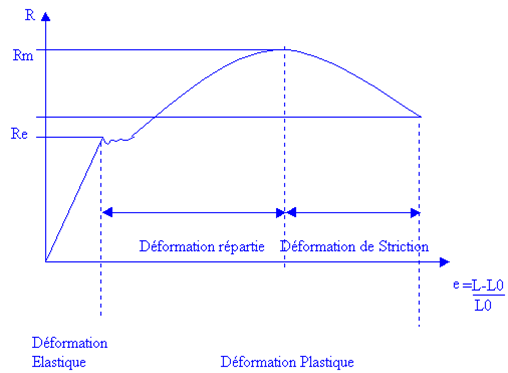
\includegraphics[width=0.8\linewidth]{img/img2}
\end{center}
}}

{\frame{
\frametitle{Diagramme conventionnel de traction}

\begin{center}
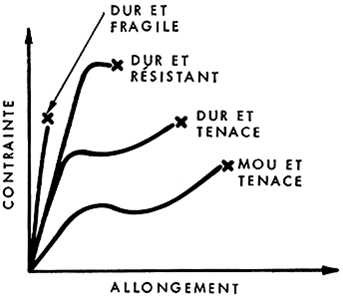
\includegraphics[width=0.48\linewidth]{img/img3} \hfill
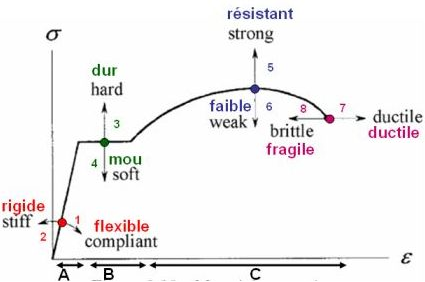
\includegraphics[width=0.48\linewidth]{img/img4}
\end{center}
}}

{\frame{
\frametitle{Diagramme conventionnel de traction}

\begin{itemize}
 \item \textbf{Ductilité}
 
La ductilité est déterminée à partir du comportement durant la striction
\begin{itemize}
 \item Si $Z$ est grand ($>0,5$) alors, le matériau est ductile,
 \item Si $Z$ est faible ($<0,1$) alors, le matériau est semi-fragile,
 \item Pour les matériaux fragiles, la rupture a lieu dans le domaine élastique
\end{itemize}

 \item \textbf{Ténacité}

La ténacité peut être définie comme le travail nécessaire  par unité de volume pour provoquer la rupture.

\begin{center}
$\frac{dW_e}{dv}=\int_0^{\epsilon_r} \sigma.d\epsilon$
\end{center}

\end{itemize}

\textit{Remarque}: il s'agit de l'aire sous la courbe rationnelle jusqu'au point de rupture.

}}

{\frame{
\frametitle{Exemple essai de traction}

\begin{center}
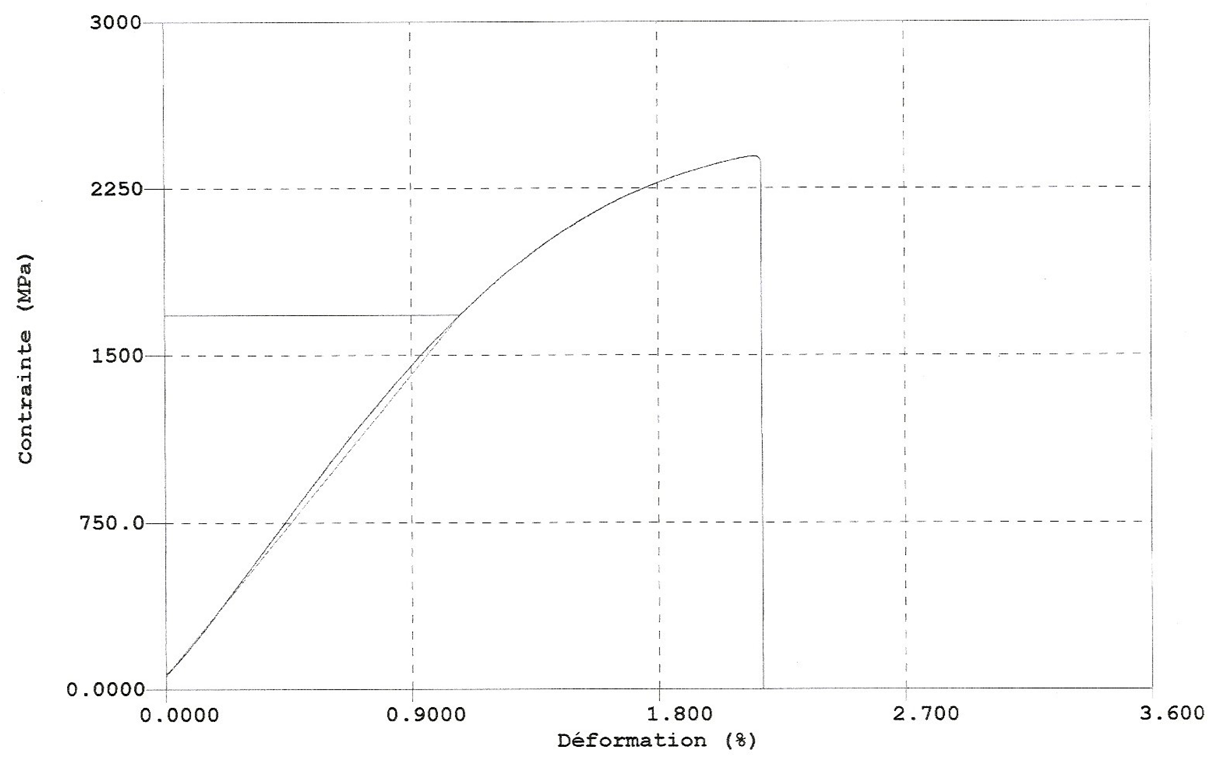
\includegraphics[width=0.8\linewidth]{img/img5}
\end{center}
}}

\section{Essai de dureté}

{\frame{
\frametitle{Essai de dureté}

\begin{itemize}
 \item La \textbf{dureté} d'un matériau définit la résistance qu'oppose une surface de l'échantillon à la pénétration d'un corps plus dur, par exemple la bille ou la pointe d'un duromètre. Des essais de rebondissement ou de pénétration sont utilisés pour caractériser la dureté des métaux, des matières plastiques et des élastomères.
 \item Il existe différents types d'essais pour caractériser la dureté. Seuls les essais de pénétration vont être présentés:
 \begin{enumerate}
  \item Brinell (NF EN 10003-1 à 3),
  \item Vickers,
  \item Rockwell (NF EN 10109-1 à 3).
 \end{enumerate}
\end{itemize}
}}

{\frame{
\frametitle{Essai de dureté}

\begin{tabular}{|c|c|c|}
\hline
Brinell & Vickers & Rockwell \\
\hline
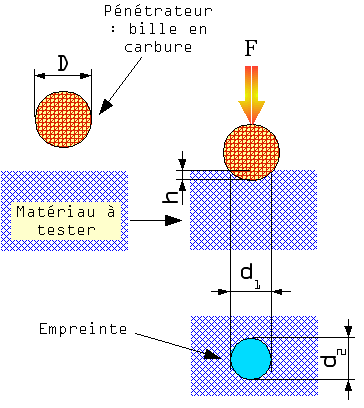
\includegraphics[width=3cm]{img/img6} & 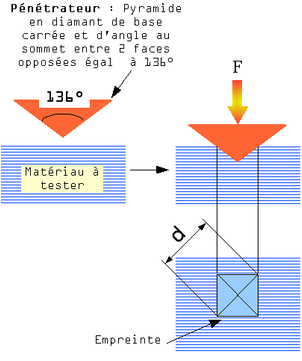
\includegraphics[width=3cm]{img/img7} &
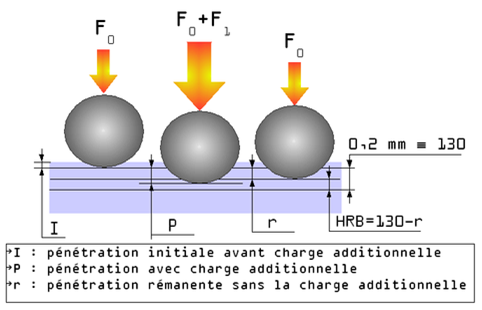
\includegraphics[width=3cm]{img/img8} \\
$d=\frac{d_1+d_2)}{2}$ & $d=\frac{d_1+d_2)}{2}$ &  \\
$h=\frac{D-\sqrt{D^2-d^2}}{2}$ &  & \\
$HBS=HBW=\frac{0,102.2.F}{\pi.D.(D-\sqrt{D^2-d^2}}$ & $HV=0,189.\frac{F}{d^2}$ & $HRO=N-\frac{h}{S}$\\
\hline
\end{tabular}
}}

{\frame{
\frametitle{Essai de dureté}

\begin{tabular}{|c|c|c|}
\hline
Brinell & Vickers & Rockwell \\
\hline
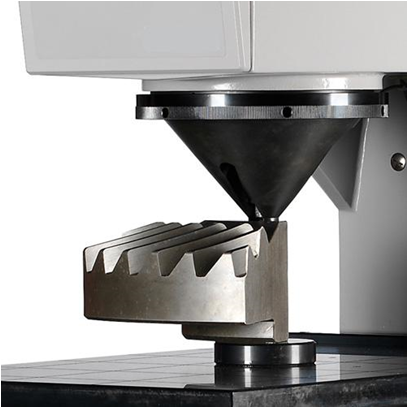
\includegraphics[width=3cm]{img/img9} & 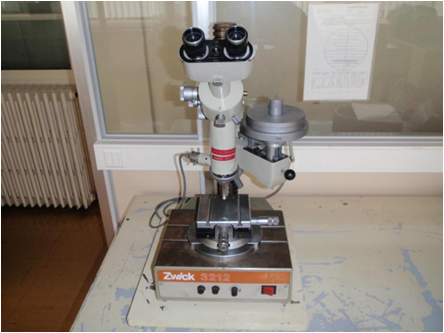
\includegraphics[width=3cm]{img/img10} &
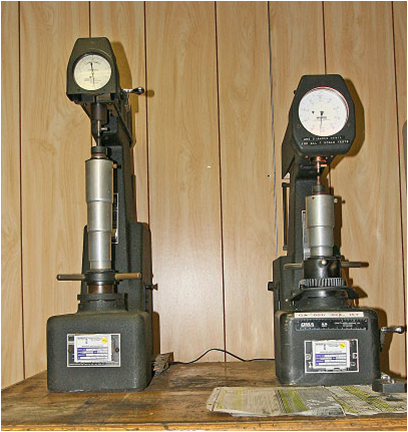
\includegraphics[width=3cm]{img/img11} \\
\hline
\end{tabular}
}}

\section{Essai de résilience}

{\frame{
\frametitle{Essai de résilience}

\begin{itemize}
 \item La connaissance des caractéristiques mécaniques déduites de l'essai de traction peut être insuffisante: des ruptures peuvent être obtenues en dessous de la limite élastique.
 \item Les paramètres de ténacité déterminés par l'essai de traction n'ont plus de sens lorsque la charge s'applique très rapidement, par \og choc \fg ($t_{charge}<1/100s$),
 \item La résistance au choc ou résilience est caractérisée par le quotient de l'énergie nécessaire pour rompre l'éprouvette en un seul coup par l'aire de la section rompue.
\end{itemize}


\begin{center}
\begin{tabular}{|c|c|}
\hline
Eprouvette en U & Eprouvette en V \\
\hline
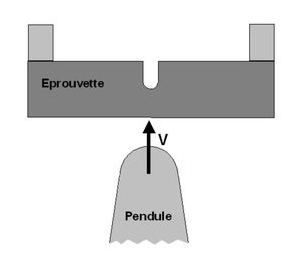
\includegraphics[width=2.5cm]{img/img12} & 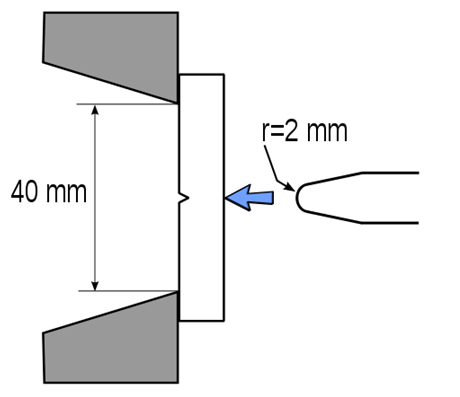
\includegraphics[width=2.5cm]{img/img13} \\
\hline
\end{tabular}
\end{center}
}}

{\frame{
\frametitle{Déroulement de l'essai de résilience}

\begin{minipage}{0.6\linewidth}
\begin{enumerate}
 \item Le couteau est écarté de la verticale à une hauteur correspondant à une énergie de départ $W_0=300J$,
 \item Le couteau est libéré. Dans sa chute, en passant à la verticale, il brise l'éprouvette,
 \item La mesure de la hauteur à la quelle remonte le pendule permet de calculer l'énergie non absorbée $W_1$,
 \item L'énergie absorbée est alors $W=W_0-W_1=W=P(h_0-h_1)$
\end{enumerate}
\end{minipage}
\hfill
\begin{minipage}{0.3\linewidth}
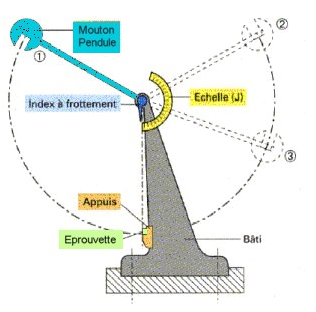
\includegraphics[width=3cm]{img/img14} \\
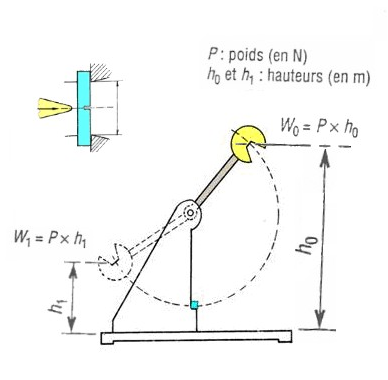
\includegraphics[width=3cm]{img/img15}
\end{minipage}
}}

\section{Essai de fatigue}

{\frame{
\frametitle{Essai de fatigue}

\begin{itemize}
 \item Un matériaux métallique soumis à des cycles répétés d'efforts subit des modifications dans ses microstructures.
 \item Une pièce ou une structure soumise à des contraintes cycliques (millions de cycles) peut rompre sous des sollicitations inférieures à la charge maximale $Rm$ ou bien souvent inférieure à la limite élastique $Re$,
 \item Un essai supplémentaire doit alors être utilisé, il sa'git de l'essai de fatigue.
\end{itemize}
}}

{\frame{
\frametitle{Déroulement de l'essai de fatigue}

\begin{minipage}{0.6\linewidth}
\begin{itemize}
 \item L'essai consiste à soumettre une série d'éprouvettes à des cycles répétitifs de sollicitations.
 \item Plusieurs types d'essais de fatigues peuvent être distingués selon le type de sollicitation à savoir : 
 \begin{itemize}
  \item fatigue en traction-compression,
  \item fatigue en torsions alternées,
  \item fatigue en flexion.
 \end{itemize}
 \item Généralement les sollicitation sont appliqués d'une façon sinusoïdale en fonction du temps.
 \item Le nombre de cycles $N$, vaut $Nf$ à la rupture.
\end{itemize}
\end{minipage}
\hfill
\begin{minipage}{0.3\linewidth}
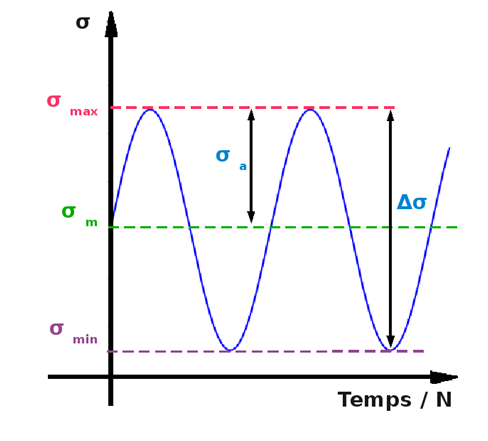
\includegraphics[width=3cm]{img/img16}
\end{minipage}
}}

{\frame{
\frametitle{Solicitations de fatigue}


\begin{minipage}{0.6\linewidth}
\begin{itemize}
 \item $\Delta \sigma=\sigma_{max}-\sigma_{min}$,
 \item $\sigma_a=\frac{\sigma_{max}-\sigma_{min}}{2}$,
 \item $\sigma_m=\frac{\sigma_{max}+\sigma_{min}}{2}$,
 \item $R \sigma=\frac{sigma_{min}}{\sigma_{max}}$.
   \end{itemize}
\end{minipage}
\hfill
\begin{minipage}{0.3\linewidth}
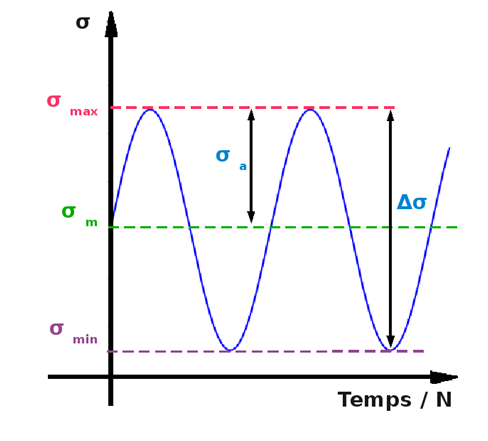
\includegraphics[width=3cm]{img/img16}
\end{minipage}

Contraintes:
\begin{tabular}{|c|c|c|c|}
\hline
Alternées symétriques & $R_{\sigma}=1$ & $\sigma_{max}=-\sigma_{min}$ & $\sigma_{m}=0$ \\
\hline
Alternées dissymétriques & $-1<R_{\sigma}<0$ & $\sigma_{max}=-\sigma_{min}$ & $0<\sigma_{m}<\sigma_{a}$ , $\sigma_{min}<0$ \\
\hline
Répétés & $R_{\sigma}=0$ & $\sigma_{m}=\sigma_{a}$ & $\sigma_{min}=0$ \\
\hline
Ondulées & $R_{\sigma}>0$ & $\sigma_{m}>\sigma_{a}$ & $\sigma_{min}>0$ \\
\hline
\end{tabular}
}}

{\frame{
\frametitle{Courbe de Wöhler}
\begin{itemize}
 \item Elle visualise la tenu d'un matériau pour un mode de sollicitation donné. Elle représente la relation expérimentale entre $\sigma_{max}$ et $Nf$. La courbe de Wöhler correspond à la valeur médiane de $N$ (50\% de survie à une contrainte donnée).
 \item Courbe de Wöhler d'un acier doux:
\end{itemize}

\begin{center}
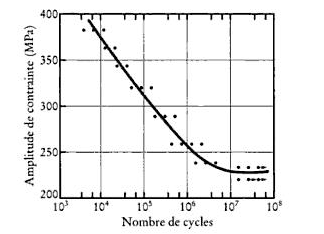
\includegraphics[width=3cm]{img/img17}
\end{center}
}}

\section{Essai de flexion}

{\frame{
\frametitle{Essai de flexion}
\begin{itemize}
 \item L'essai de flexion 3 points décrit dans l'ISO 178 et l'ASTM D 790 représente les méthodes de caractérisation classiques pour les plastiques rigides et semi-rigides.
 \item Les résultats typiques incluent le Module de Young (module de flexion), la contrainte à l'allongement 3,5\% de même que les contraintes et allongements sur le point d'élasticité et à la rupture de l'éprouvette. 
\end{itemize}

\begin{center}
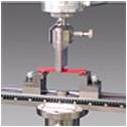
\includegraphics[width=2cm]{img/img18} \hfill
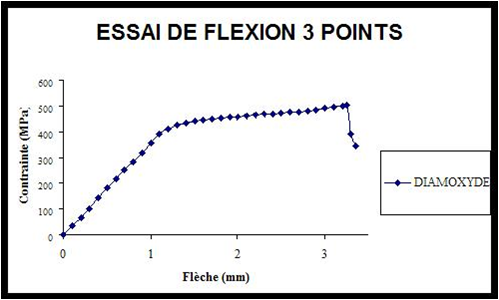
\includegraphics[width=5cm]{img/img19}
\end{center}

}}

\section{Essai de torsion}

{\frame{
\frametitle{Essai de torsion}
\begin{itemize}
 \item Il permet de caractériser le comportement d'un matériau soumis à une charge de torsion.
 \item Les résultats de l'essai de torsion sont utilisés pour tracer une courbe de contrainte/déformation.
 \item Les propriétés de cisaillement sont souvent déterminées par un essai de torsion.
\end{itemize}

\begin{minipage}{0.48\linewidth}
\begin{itemize}
 \item Caractéristiques
\begin{itemize}
 \item $E$: Module d'Young
 \item $\nu$: Coefficient de Poisson,
 \item $G$: Module de Cisaillement,
 \item $K$: Module d'élasticité isostatique.
\end{itemize}
\end{itemize}
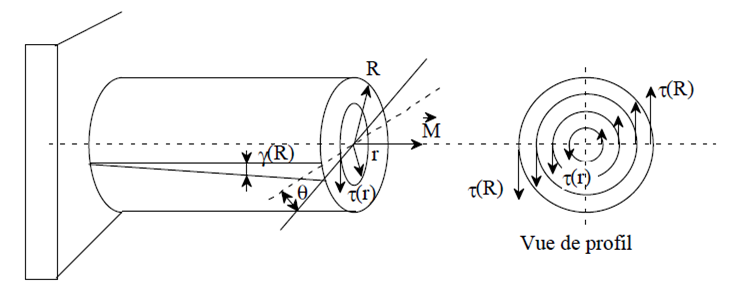
\includegraphics[width=5cm]{img/img20}
\end{minipage}
 \hfill
\begin{minipage}{0.48\linewidth}
\begin{center}
\begin{tabular}{|c|}
\hline
$\tau=G.\gamma(r)$ \\ \hline $\gamma(r)=\frac{r}{L}.\theta$ \\ \hline
$\nu=\frac{\frac{l_0-l}{l_0}}{\frac{L_0-L}{L_0}}$ \\ \hline $E=2(1+\nu).G$ \\ \hline
 $K=\frac{1}{3}.\frac{E}{(1-2.\nu)}$ \\ \hline
\end{tabular}
\end{center}
\end{minipage}
}}



{\frame{
\frametitle{Conclusion}

\begin{savoir}
Vous êtes capables :
\begin{itemize}
 \item de caractériser un matériau avec des proprités mécaniques spécifiques,
 \item de présenter l'organisation d'un essai afin de mettre en évidence ces caractéristiques.
\end{itemize}
\end{savoir}

\begin{prob}
Vous devez êtes capables :
 \begin{itemize}
 \item de connaître d'associer aux matériaux les plus classiques ces propriétés.
 \end{itemize}
\end{prob}
}}


\end{document}